% Model-based experimental design: confidence x accuracy, orthogonalised.
% Compile: pdflatex fig11_experiment.tex
\documentclass[border=6pt]{standalone}
\usepackage{amsmath,amssymb}
\usepackage{tikz}
\usetikzlibrary{arrows.meta,positioning,fit,calc}
\begin{document}
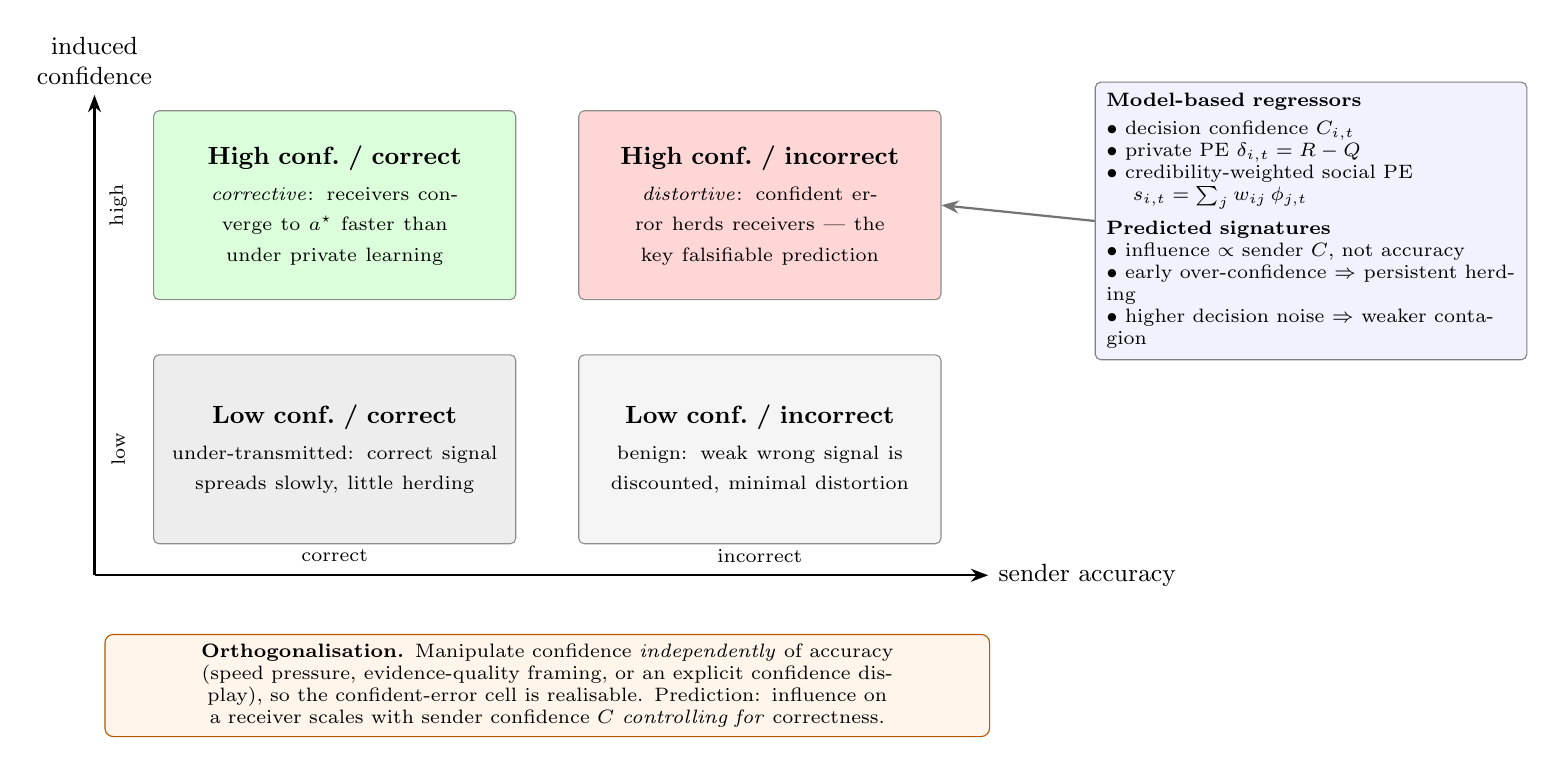
\begin{tikzpicture}[
  font=\small,>={Stealth[length=2.2mm]},
  cell/.style={minimum width=46mm,minimum height=24mm,align=center,
               draw=black!45,rounded corners=2pt,text width=42mm,inner sep=3pt},
  reg/.style={draw=black!50,rounded corners=2pt,fill=blue!5,align=left,
              text width=52mm,inner sep=4pt,font=\scriptsize},
]
% ---- 2x2 design (x: accuracy, y: induced confidence) -------------------
\node[cell,fill=green!14] (HC) at (0,0)
   {\textbf{High conf.\ / correct}\\[2pt]\scriptsize \emph{corrective}: receivers
    converge to $a^\star$ faster than under private learning};
\node[cell,fill=red!16] (HW) at (5.4,0)
   {\textbf{High conf.\ / incorrect}\\[2pt]\scriptsize \emph{distortive}: confident
    error herds receivers --- the key falsifiable prediction};
\node[cell,fill=black!7] (LC) at (0,-3.1)
   {\textbf{Low conf.\ / correct}\\[2pt]\scriptsize under-transmitted: correct
    signal spreads slowly, little herding};
\node[cell,fill=black!4] (LW) at (5.4,-3.1)
   {\textbf{Low conf.\ / incorrect}\\[2pt]\scriptsize benign: weak wrong signal
    is discounted, minimal distortion};
% axes
\draw[->,thick] (-3.05,-4.7) -- (-3.05,1.4) node[above,align=center]{induced\\confidence};
\node[rotate=90,font=\scriptsize] at (-2.75,0){high};
\node[rotate=90,font=\scriptsize] at (-2.75,-3.1){low};
\draw[->,thick] (-3.05,-4.7) -- (8.3,-4.7) node[right,align=center]{sender accuracy};
\node[font=\scriptsize] at (0,-4.45){correct};
\node[font=\scriptsize] at (5.4,-4.45){incorrect};

% ---- orthogonalisation note --------------------------------------------
\node[draw=orange!70!black,rounded corners=3pt,fill=orange!8,text width=110mm,
      align=center,font=\scriptsize] (OR) at (2.7,-6.1)
  {\textbf{Orthogonalisation.} Manipulate confidence \emph{independently} of
   accuracy (speed pressure, evidence-quality framing, or an explicit confidence
   display), so the confident-error cell is realisable. Prediction: influence on
   a receiver scales with sender confidence $C$ \emph{controlling for} correctness.};

% ---- model-derived regressors ------------------------------------------
\node[reg] (RG) at (12.4,-0.2)
  {\textbf{Model-based regressors}\\[2pt]
   $\bullet$ decision confidence $C_{i,t}$\\
   $\bullet$ private PE $\delta_{i,t}=R-Q$\\
   $\bullet$ credibility-weighted social PE\\
   \hspace*{1.2em}$s_{i,t}=\sum_j w_{ij}\,\phi_{j,t}$\\[3pt]
   \textbf{Predicted signatures}\\
   $\bullet$ influence $\propto$ sender $C$, not accuracy\\
   $\bullet$ early over-confidence $\Rightarrow$ persistent herding\\
   $\bullet$ higher decision noise $\Rightarrow$ weaker contagion};
\draw[->,thick,black!55] (RG.west) -- (HW.east);
\end{tikzpicture}
\end{document}
